%%%%% Estudio de mercado%%%%%
\section{Estudio de mercado}
\subsection{Diseño del instrumento de investigación}
Con el propósito de conocer las expectativas del mercado respecto a una aplicación para obtener dimensiones y saber si es un producto de interés; el instrumento de investigación que se diseño fue una encuesta conformada  por un total de ocho preguntas.

La encuesta es la siguiente:

\begin{center}
    \begin{tabular}{|p{16cm}|}
        \hline
            \rowcolor[rgb]{0.1,0.1,0.1} \\
            \rowcolor[rgb]{0.1,0.1,0.1} 
            \textbf{\Large{{\color{white}Fit a thing}}} \\[0.3cm]
        \hline
        	 \\
            Somos alumnos de octavo semestre, realizamos esta encuesta con el fin de conocer si la 
            aplicación a desarrollar puede satisfacer las necesidades del mercado. Tu opinión nos ayudará
            a desarrollar una mejor aplicación. Responde honestamente.\\[0.3cm]
             \textcolor{rojo}{*Obligatorio}\\[0.3cm]
        \hline
            \rowcolor[rgb]{0.8,0.8,0.8}\\
            \rowcolor[rgb]{0.8,0.8,0.8}
            \textbf{\color{darkgray}Dispositivo} \\ [0.3cm]
        \hline
            ¿Cuentas con un smartphone? \textcolor{rojo}{*}\\
            \hspace{1cm}\textit{Sí}\\
            \hspace{1cm}\textit{No}\\
            \hline
             ¿Qué sistema operativo utiliza? \textcolor{rojo}{*}\\
            \hspace{1cm}\textit{Android}\\
            \hspace{1cm}\textit{iOS}\\
        	 \hspace{1cm}\textit{Windows Phone}\\
        	 \hspace{1cm}\textit{Otro}\\
        	 \hline
    \end{tabular}
    \newpage
    \begin{tabular}{|p{16cm}|}
        	 \hline
        	 En caso de ser Android, ¿qué versión es?\\
        	 \hspace{1cm}\textit{Ice Cream Sandwich}\\
            \hspace{1cm}\textit{Jelly Bean}\\
        	 \hspace{1cm}\textit{KitKat}\\
        	 \hspace{1cm}\textit{Lollipop}\\
        	 \hspace{1cm}\textit{Marshmallow}\\
        	 \hspace{1cm}\textit{Nougat}\\
        	 \hspace{1cm}\textit{No lo sé}\\
        	 \hspace{1cm}\textit{Otra versión}\\
        	 \hline
            \rowcolor[rgb]{0.8,0.8,0.8}\\
            \rowcolor[rgb]{0.8,0.8,0.8}
            \textbf{\color{darkgray}Funcionalidad} \\ [0.3cm]
            ¿Has utilizado u oído de alguna de las siguientes aplicaciones? \textcolor{rojo}{*}\\
            \hspace{1cm}\textit{3D Plomada} \textbf{[Sí/No]}\\
            \hspace{1cm}\textit{Smart Distance} \textbf{[Sí/No]}\\
        	 \hspace{1cm}\textit{Smart Measure} \textbf{[Sí/No]}\\
	 \hline
	 ¿Conoces alguna aplicación para tomar dimensiones (altura, ancho y/o largo), que no se mencione
	  en la pregunta anterior?¿Cuál?\\
	  \hline
	  ¿Piensas que sería útil poder tomar dimensiones (altura, ancho y/o largo) de objetos
	   (p.e. muebles, puertas, árboles, etc.) con tu smartphone?\textcolor{rojo}{*}\\
	   \hspace{1cm}\textit{Sí}\\
	   \hspace{1cm}\textit{No}\\
	   \hspace{1cm}\textit{Tal vez}\\
	   \hline
	   ¿Utilizarías una aplicación que calcule las dimensiones de los objetos con solo tomar fotos?\textcolor{rojo}{*}\\
	   \hspace{1cm}\textit{Sí}\\
	   \hspace{1cm}\textit{No}\\
	   \hspace{1cm}\textit{Tal vez}\\
	   \hline
	\rowcolor[rgb]{0.8,0.8,0.8}\\
            \rowcolor[rgb]{0.8,0.8,0.8}
            \textbf{\color{darkgray}Danos tu opinión} \\ [0.3cm]
            ¿Qué debería tener una aplicación para capturar medidas?\\
            \hline
    \end{tabular}
    \end{center}
\newpage 

\subsection{Análisis de resultados}
La encuesta se aplicó a un total de 93 personas, obteniendo los siguientes resultados.
    \begin{enumerate}
        \item \textbf{¿Cuentas con un smartphone?}\\
        La mayor parte de los encuestados (95,0\%) cuenta con un smartphone. Lo que significa que los smartphone son dispositivos de uso cotidiano.\\
        \begin{figure}[h!]
	        \centering	            
	        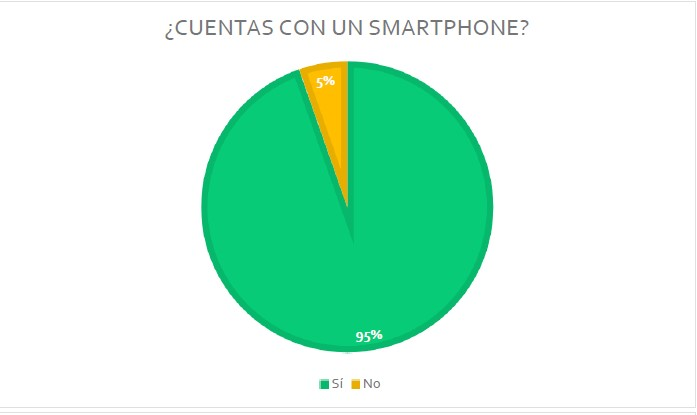
\includegraphics[width=15.5cm]{IMG/Graficas/1}
	            \caption{ \textbf{Pregunta 1. Fuente: Elaboración propia.}}
	            \label{fig:edomercado1}
	\end{figure}
	\newpage
	
        \item \textbf{¿Qué sistema operativo utiliza?}\\
        El 85,0\% de los encuestados que contaban con smartphone utilizan Android, convirtiendo lo en el Sistema Operativo preferido. Así que desarrollar la aplicación para Android nos permite abarcar a un mercado más amplio.
        \begin{figure}[h!]
	        \centering	            
	        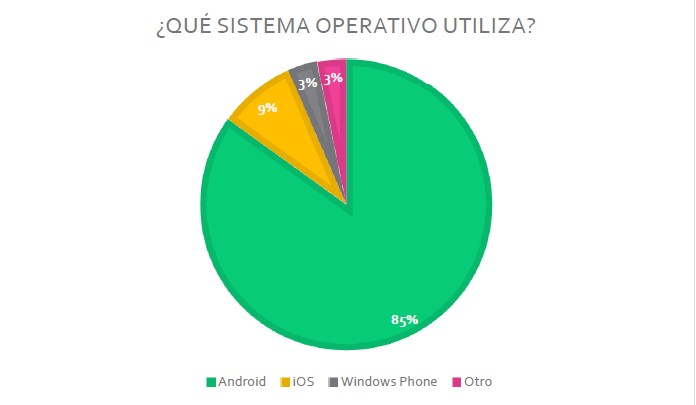
\includegraphics[width=15.5cm]{IMG/Graficas/2}
	            \caption{ \textbf{Pregunta 2. Fuente: Elaboración propia.}}
	            \label{fig:edomercado2}
	\end{figure}
	\newpage
	
        \item \textbf{En caso de ser Android, ¿qué versión es?}\\	
        En esta pregunta se observa que el 24,0\% de los encuestados desconoce la versión de Android que están utilizando. El 18,0\% utiliza alguna de las versiones anteriores a Lollipop. Y el 58,0\% restante utiliza Lollipop o alguna version posterior a este, es decir, más de la mitad de los usuarios Android cuentan con Lollipop o una versión más reciente, lo cual nos ayuda a garantizar que el dispositivo contará con las especificaciones necesarias (contar con acelerómetro y tener una cámara con 5 o más megapixeles)  para el funcionamiento de nuestra aplicación.
        \begin{figure}[h!]
	        \centering	            
	        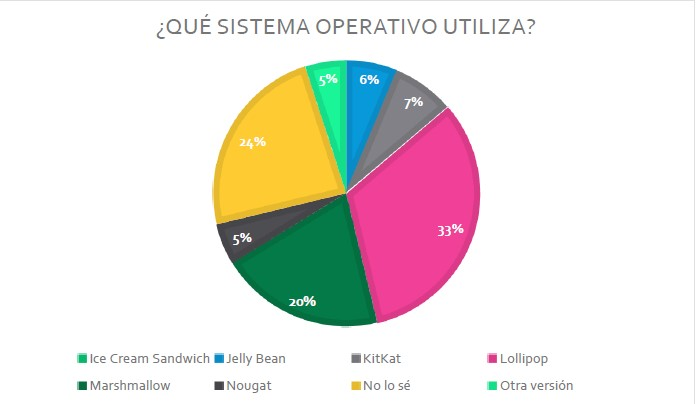
\includegraphics[width=15.5cm]{IMG/Graficas/3}
	            \caption{ \textbf{Pregunta 3. Fuente: Elaboración propia.}}
	            \label{fig:edomercado3}
	\end{figure}
	
        \item \textbf{¿Has utilizado u oído de alguna de las siguientes aplicaciones?}\\
        Vemos que pocas personas han utilizado aplicaciones similares a la que se pretende desarrollar. Lo cual indica que será difícil introducirla en el mercado.
        
        \item \textbf{¿Conoces alguna aplicación para tomar dimensiones (altura, ancho y/o largo), que no se mencione en la pregunta anterior?¿Cuál?}\\
	    Solo un encuestado respondió conocer alguna otra aplicación, ''Meter Measure''.
	    \newpage
	    
	    \item \textbf{¿Piensas que sería útil poder tomar dimensiones (altura, ancho y/o largo) de objetos (p.e. muebles, puertas, árboles, etc.) con tu smartphone?}\\
	    El 60,0\% de los encuestado piensa que podría ser útil una aplicación de este tipo, el 30,0\% considera que tal vez y el 10,0\% restante piensa que no.
	    \begin{figure}[h!]
	        \centering	            
	        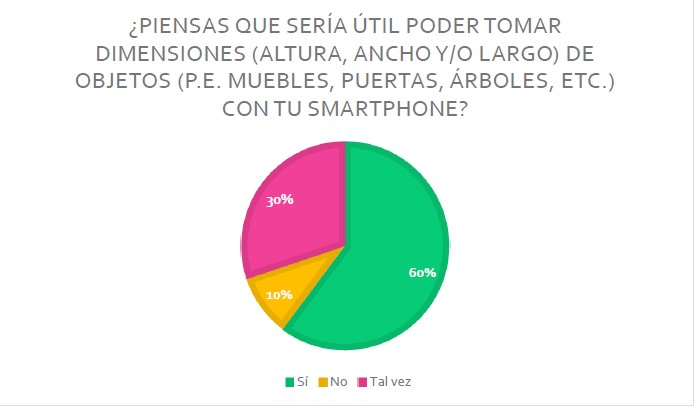
\includegraphics[width=15.5cm]{IMG/Graficas/4}
	            \caption{ \textbf{Pregunta 6. Fuente: Elaboración propia.}}
	            \label{fig:edomercado4}
	\end{figure}
	\newpage
	
	    \item \textbf{¿Utilizarías una aplicación que calcule las dimensiones de los objetos con solo tomar fotos?}\\
	    El 61,0\% dice que utilizaría una aplicación de este tipo, el 26,0\% que tal vez y el 13,0\% restante que no. A pesar de que en las preguntas 4 y 5 vemos que aplicaciones de este tipo no son conocidas ni utilizadas el 87,0\% consideraría el utilizar la nuestra.
	    \begin{figure}[h!]
	        \centering	            
	        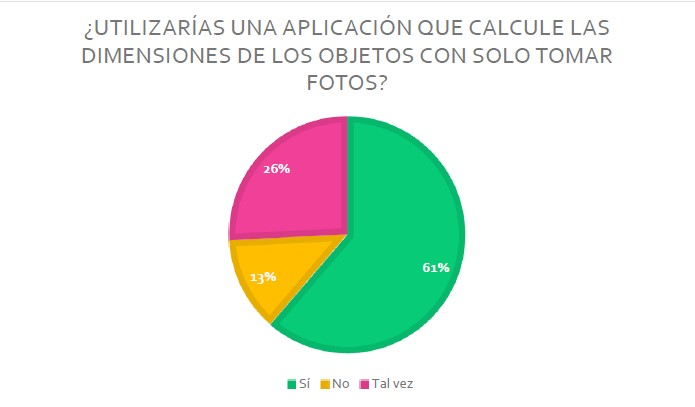
\includegraphics[width=15.5cm]{IMG/Graficas/5}
	            \caption{ \textbf{Pregunta 7. Fuente: Elaboración propia.}}
	            \label{fig:edomercado5}
	\end{figure}
	
	    \item \textbf{¿Qué debería tener una aplicación para capturar medidas?}\\
	    Entre las respuestas que más se econtrarón están:
	    \begin{itemize}
	    \item Ser precisa.
	    \item Reconocer objetos de manera automática.
	    \item Tener conversión de medidas.
	    \item Ser de fácil uso.
	    \item Tener una interfaz sencilla.
	    \item Poder guardar los resultados de las mediciones.
	    \end{itemize}
    \end{enumerate}
	